\documentclass[aps,pre,reprint,superscriptaddress,amsmath,amssymb,nofootinbib]{revtex4-1}
\usepackage{graphicx}
\usepackage{dcolumn}
\usepackage{bm}
\usepackage{hyperref}
\usepackage{natbib}
\renewcommand{\thefootnote}{\fnsymbol{footnote}}
\DeclareGraphicsExtensions{.pdf}

\begin{document}

\title{Plum pudding model for growing small-world networks}
\author{Ari Zitin}
\affiliation{Institute for Research in Electronics and Applied Physics, University of Maryland, College Park, Maryland 20742, USA}
\author{Alex Gorowara}
\affiliation{Institute for Research in Electronics and Applied Physics, University of Maryland, College Park, Maryland 20742, USA}
\author{Shane Squires}
\affiliation{Institute for Research in Electronics and Applied Physics, University of Maryland, College Park, Maryland 20742, USA}
\affiliation{Department of Physics, University of Maryland, College Park, Maryland 20742, USA}
\author{Mark Herrera}
\affiliation{Institute for Research in Electronics and Applied Physics, University of Maryland, College Park, Maryland 20742, USA}
\affiliation{Department of Physics, University of Maryland, College Park, Maryland 20742, USA}
\author{Tom Antonsen}
\affiliation{Institute for Research in Electronics and Applied Physics, University of Maryland, College Park, Maryland 20742, USA}
\affiliation{Department of Electrical and Computer Engineering, University of Maryland, College Park, Maryland 20742, USA}
\affiliation{Department of Physics, University of Maryland, College Park, Maryland 20742, USA}
\author{Michelle Girvan}
\affiliation{Institute for Research in Electronics and Applied Physics, University of Maryland, College Park, Maryland 20742, USA}
\affiliation{Institute for Physical Science and Technology, University of Maryland, College Park, Maryland 20742, USA}
\affiliation{Department of Physics, University of Maryland, College Park, Maryland 20742, USA}
\author{Edward Ott}
\affiliation{Institute for Research in Electronics and Applied Physics, University of Maryland, College Park, Maryland 20742, USA}
\affiliation{Department of Electrical and Computer Engineering, University of Maryland, College Park, Maryland 20742, USA}
\affiliation{Department of Physics, University of Maryland, College Park, Maryland 20742, USA}

\date{\today}

\begin{abstract}
Researchers have studied spatially embedded complex networks which are static in time, but networks in nature are inherently dynamical, gaining links and nodes as they develop over time. 
We explore the properties of growing networks, investigating the relationship between statistical network properties and the space in which they are embedded. 
In particular, we consider a class of models in which nodes are place one by one in random locations in space and, after placement, form connections with nearby nodes. 
We find that the resulting networks are small-world networks, and we characterize how spatial embedding supports the emergence of small-world properties.
\end{abstract}

\pacs{05.45.-a, 05.65.+b, 89.75.-k, 89.75.Fb ,89.75.Hc} %Nonlinear dynamics and chaos, Self-organized systems, Complex Systems, Structures and organization in complex systems, Networks and genealogical trees

\maketitle

\section{INTRODUCTION}
%in the introduction don't forget to present definitions we use, in particular be clear what we mean by small world property
%mention how our generalizations were chosen for their physical significance rather than the ease with which we can perform comupational and analytic calculations of their properties. 

\section{THE OHO MODEL}
The Ozik-Hunt-Ott (OHO) model, presented in \cite{ozik2004}, considers a network which initially has a clique of $m+1$ nodes on the circumference of a circle. 
At each discrete time step the network is grown according to the following rules: 
(1) a new node is placed at a randomly selected point on the circumference of the circle;
(2) the new node is linked to its $m$ nearest neighbors;
(3) steps (1-2) are repeated until the network has $N$ nodes.
Since the network is incremented in size by one node each timestep, the network size $N$ can also be used as the system time parameter.  
It has been shown \cite{ozik2004} that this growth model leads to a small-world network with an exponentially decaying degree distribution. 
The original goal of the OHO model was to explore the effect that geographic locality has on the growth of networks; in this paper, we extend this analysis by considering networks growing by geographic attachment preference in more general Euclidean spaces. 

The original OHO model exhibits the following three properties which indicate that the small-world property is present:
\begin{description}
  \item[Degree Distribution] The degree distribution $H(k)$ is the probablility that a node with have $k$ network connections at time $N$.
For large $N$, the degree distribution of the OHO model is given by 
\begin{equation}
H(k) = \frac{1}{m+1}\left(\frac{m}{m+1}\right)^{k-m}
\end{equation}
for $k \geq m$ and $H(k) = 0$ for $k < m$ \cite{ozik2004}.
The average node degree $\langle k \rangle$ is $2m$.
Since the average node degree remains finite even as $N \to \infty$, the OHO model meets the first criterion for the small-world property.
  \item[Characteristic Path Length] The characteristic path length $\ell$ is the average of the length of the shortest path between two randomly selected nodes.
In the OHO model, simulation results allow the verification of the desired small world path lenth scaling; $\ell \sim \log N$.
This may be explained intuitively by noting that as new nodes are added they push apart the older connected nodes, lengthening the distance traversed by older edges. 
These older nodes then serve as hubs for travel between pairs of nodes across the network, dramatically decreasing the shortest path length between any given pair of nodes.
  \item[Clustering Coefficient] The final criterion for a small world network is a nonzero clustering coefficient as $N \to \infty$. 
The clustering coefficient of a network is the fraction of connected triples in a network which are also traignles.
This measures whether two nodes which are both connected to a third node are likely to be connected to one another \footnote{In \cite{ozik2004} an alternate definition of clustering was used, specifically the average of the local clustering $C_i$ of each node, $C_i = \frac{q_i}{\frac{1}{1} k_i (k_i-1)}$ where $q_i$ is the number of links between the $k_i$ neighbors of node $i$.}
\end{description}
Thus the OHO model produces a small-world network.
Here, we hypothesize that the small-world properties are caused by the fact that, although new edges are all local, nearby nodes separate over time, creating long-range connections.
To test this hypothesis we investigate generalizations to higher-dimensional spaces in order to explore how the small-world property emerges in dynamically growing spatially embedded networks.

\section{The Thomson Problem}
The natural generalization from embedding nodes on the one-dimensional circumference of a circle is to embed them on the two-dimensional surface of a sphere, or in general on the $d$-dimensional surface of a hypersphere.
On a circle it is trivial to arrange $N$ points along the circumference with uniform spacing, but the analogous procedure is much more difficult on higher dimensional surfaces.
One way to generalize the procedure is to consider each node to be a point charge on the surface of a $d$-dimensional conductor and find their equilibrium configuration. 
The problem of finding the equilibrium configuration of points on the surface of a sphere dates back to 1904 when J.J. Thomson introduced his plum pudding model of the atom, in which a centroal could of positive charge was surrounded by a discrete negative charges on the surface \cite{thomson1904}
A key problem for him was arranging the electrons (corpuscles) on the surface of the sphere of pudding such that the potential energy is minimized.

Here we adopt the thomson problem as one possible generalization of the OHO model.
We model the nodes as point charges confined to exist on the surface of a sphere of unit radius.
%In this way we produce a configuration of nodes on the sphere's surface such that each internode area interval is approximately (up to numerical defects) equal, implying that if we were to select a point on the sphere uniformly at random, each area interval would be equally likely to be selected.
Now at each timestep we drop a node into an area interval selected at random on the sphere and add links to connect it to its $m$ nearest neighbors, where here distance is defined as the shortest great circle path along the surface of the sphere between two nodes.
Next we require that the potential energy between the nodes is minimized.
For large $N$, the repulsive interaction ensures that the points are distributed approximately uniformly across the surface of the sphere.
In this way we reproduce the key features of the OHO model, a growing network with new nodes only making local connections, but we also introduce a new parameter, the dimension of the space in which the growing network is embedded.
In the following sections we explore the differences between the OHO model and the higher dimension generalizations.

%FIXME rethink how we integrate this with the higher dimensional stuff, may have to rewrite most of this section!
\subsubsection{The 2D Case: Network Embedded on the Surface of a Sphere}
The first generalization we explore is the case of nodes confined to exist on the surface of a unit sphere in Euclidean 3-space.
This is directly analogous to the original Thomson problem presented in \cite{thomson1904}, where $N$ electrons are bound to the surface of a sphere and interact with each other via the Couloumb force.
As a result of the Couloumb interaction, the minimum energy configuration for these points on the sphere is one where the points are distributed in an approximately uniform manner across the surface of the sphere.
In order to determine if this model produces a small world network we determine the following three properties:
\begin{description}
  \item[Degree Distribution] The uniform distribution of nodes on the surface of the sphere leads to a uniform probability of choosing an area interval in which to place a new nodes; thus existing nodes each have an equal probability of having their degree increased at each timestep.
This causes the degree distribution for this new model to be identical to the degree distribution for the original OHO model, for more detail on this discussion refer to the section on invariant properties at the end of this article.
  \item[Characteristic Path Length] For this model we find that the the average shortest path length $\ell$ scales logarithmically with the network size $N$, that is, $\ell \sim \log N$. 
This is a reasonable result because as the network grows in size the older nodes get pushed apart by the repulsive Coulumb force thus leaving bridges across the network that span a significant physical distance.
These long range links serve to connect disparate regions of highly interconnected nodes, dramatically reducing the shortest path length between any two nodes in the network.
At each timestep only geographically local connections are made, but due to the dynamic nature of the nodes' spatial positions, each timestep can make existing links longer in physical space, thus building bridges across the network.
Furthermore, we find that for a given value of $N$ the shortest path between any two nodes in this 2D case is shorter than that of the corresponding 1D case (the original OHO model).
One possible explanation for this feature is that the surface of a sphere provides more freedom for nodes to move around each other, thus increasing the chance that a shortcut is created.
In the original OHO model each node, like a boson in a Tonks-Girardeau gas, is forever locked between its two original spatial neighbors, and thus long range links can only be created if new nodes are placed between the two neighbors.
In this first generalization of the OHO model, the repulsive Couloumb force between electrons allows them to rearrange thier relative positions by moving in 2 dimensions in order to minimize the potential energy of the configuration.
Thus two originally adjacent nodes can be moved apart around other nodes, forming long range links; of course placing new nodes between them will also create bridges, but these effects combine to produce shorter path length in the 2D case than in the 1D case.
  \item[Clustering Coefficient] 
%I'm going to leave this section blank until we have results and figures for this since that should determine what we write.
\end{description}
Thus we find that that the model of a network growing on the surface of a sphere with geographic attachment preference leads to the emergence of the small-world property.
We now move onto discussing the generalized case of a network embedded on the surface of a $d$-sphere in order to see how the dimension of the embedding space impacts the network properties.

\subsubsection{Spatial Embedding of Networks on the Surface of the Unit $d$-Sphere}
In this extension of the OHO model, we generalized from the simple case of nodes on a circle and investigated the possibility of placing nodes on a $d$-dimensional sphere.
In order to preserve the non-preferential selection of the OHO model, favoring no inter-node interval above others, we placed new nodes with uniform probability on the surface of the $d$-sphere after "relaxing" the preexisting nodes into a roughly homogenous distribution. 
For the relaxation, we treated each node as a point charge, and used a gradient-descent algorithm to let the repulsive forces between nodes move them to an approximate equilibrium.

For the case of a $d$-dimensional sphere embedded in $d+1$-dimensional space, we used the Coulomb force law appropriate to a $d$-dimensional space, treating the sphere as a curved universe containing bodies acting in accordance with $d$-dimensional laws rather than an arbitrary limitation on a $d+1$-dimensional universe.  
As we explain below, the conformity of these spherical networks to the appropriate degree distribution indicates that this is a sound method for relaxing nodes into a homogenous distribution.

\section{THE PLUM PUDDING MODEL}
A key feature of the OHO model is that the nodes can only be placed on the circumference of a circle. 
When we generalize this to higher dimensions we are still embedding the network on a $d$-dimensional surface in a $d+1$ dimensional space, so nodes never occupy a volume in the embedding space.
In this generalization we explore how the network properties are affected if we instead embed a growing network in a $d$-dimensional space without restricting them to a spherical shell.  
In order to ensure unbiased behavior over all nodes, we instead confine them to a $d$-dimensional ball. 

In this case, we can generalize the main features of the OHO model in another way, inspired by Thomson's plum pudding model.
We model our network as a collection of classical electrons, each electron representing a node, free to move around in a ``cloud" of positive charge of uniform density, filling a $d$-dimensional ball of unit radius.
The repulsive potential between nodes ensures that they are spaced approximately equidistantly for large $N$ in the minimum potential configuration, while the cloud of positive charge ensures that the nodes do not move arbitrarily far from some fixed starting point.
%FIXME deal with force law issues before editing this and subsequent sections
Due to the nature of Gauss' Law in different dimensions we find that for each dimension the potential between any given node and the cloud of positive charge is proportional to the square of the distance between the center of the embedding volume and the node in question.
This means that we can visualize this model as a collection of classical electrons all connected to some origin point by springs (a harmonic potential) and interacting with each other via the dimensionally appropriate Couloumb force.  
In order to maintain the unit $d$-ball, this potential is kept proportional to the number of nodes in the graph, and in the Plum Pudding analogy can be said to have a "charge" equal and opposite to the sum of "charges" over all of its nodes.
Like the OHO model we place new nodes randomly in the volume and connect them to their $m$ nearest neighbors, where here we define nearest to be the Euclidean distance between the nodes.
After each node is placed, the configuration is rearranged in order to minimize the total potential energy of the system, which forces the nodes to arrange themselves in an approximately uniform distribution throughout the volume in the embedding space.

%should we include a picture of the 2D Plum Pudding with age colored? It's a good picture, but I'm just not sure how relevant it is.


\subsection{Boundary Conditions on the OHO Model}
First we consider the low-dimensional cases and compare them to the original OHO model and its generalizations to see how these models differ.
The key difference is that when we embed networks on a smooth surface like in the previous models there are no hard boundaries beyond which the nodes cannot move.
In the plum pudding model on the other hand, if nodes move too far from the origin (the center of the volume in which the nodes are embedded) they hit a potential boundary beyond which they cannot pass.
These boundary conditions lead to differences in network properties such as the clustering coefficient between the two models (plum pudding model and the generalized OHO model).

\subsubsection{The 1D Case: Nodes on a Line}
The laws of electromagnetism in 1 dimension lead to a constant force term between each electron, and thus this case is really just a line segmented into equal parts by the set of nodes. 
This model is essentially the same as the original OHO model (nodes on the circumference of a circle), with the exception of a boundary condition. 
On the circle each node borders two internode intervals while on the line the nodes at each endpoint only border one internode interval.
Thus this model leads to nearly identical results as the OHO model, especially for large $N$.
For large $N$ there are still only two boundary nodes, but they make up a fraction $\frac{2}{N}$ of all the nodes, and thus barely contribute to the stastical network properties.
For very small values of $N$ we see some minor differences between the two model, but for any value of $N$ large enough to calculate statistics we find agreement between the 1D Plum Pudding model and the original OHO model (which is the 1D case of the generalized thomson model discussed earlier).

%What properties should we include here? We have to put some plots up, maybe comparing 1D PP and TP?


\subsubsection{The 2D Case: Nodes on a Disk}
Although the disk is a 2 dimensional object and the sphere is fundamentally a 3 dimensional object, nodes embedded on the surface of a sphere and nodes embedded on a disk both live in an effectively 2 dimensional space.
As a result we would expect that the properties explored for the case of nodes embedded on the surface of a sphere hold in this case as well.
Since the minimum energy configuration for the nodes in a cloud of positive charge is a uniform distribution across the face of the unit circle, we expect to find an identical degree distribution to that of the prior models.
This is verified and discussed in more depth in the section on invariant properties at the end of this article.
%include some stuff about how clustering and path length look different from sphere if we don't choose the appropriate force law. Perhaps include more about how the force law impacts the properties? 

\subsection{Spatial Embedding of Networks in a unit $d$-Ball}
Similar to the $d$-sphere, the $d$-ball, a region embedded in $d$-dimensional space, is a generalization of the simpler models to higher dimensions.  
However, there is an important distinction: while the repulsive forces between nodes still act as $F \propto \frac{1}{r^{d-1}}$, the attractive force - the contribution of the "cloud" of positive charge - is independent of dimension.  
This is the proper result for such a scenario, however; Gauss's law continues to hold in the same general form in higher dimensions.

And, because of the balance between the repulsive and attractive forces, the nodes were kept naturally confined to a unit $d$-dimensional ball, without resort to artificial boundary conditions.  
The force did, however, level off at the edge of the $d$-ball, in order to prevent oscillatory effects for small $N$ with large timesteps.  
The arrangement of nodes is best seen in the case of the 2-ball, the most photogenic of $d$-balls.  

\section{INVARIANT PROPERTIES}
Several important network features can be found analytically and do not depend on dimension or on the choice of the plum pudding or Thomson model.
A key observation in each of the following derivations is that the probability that each newly added node will form an edge to any particular existing node is $\frac{m}{N}$ for all nodes.
This is because existing nodes are distributed approximately uniformly, and new nodes are placed randomly according to a uniform distribution.

\subsection{Degree Distribution}
Here we show that for each considered model, we produce the same master equation governing the evolution of the degree distribution (in particular the master equation for the degree distribution in \cite{ozik2004}).  
This master equation is not specific to the spatial structure of the network, or indeed the existence of any spatial structure, but rather relies on the uniform distribution of new links among preexisting nodes.  
It appears, in various forms, in networks such as the Deterministic Uniform Random Tree \cite{zhang2008topologies}.

We define $\hat{G}(k,N)$ to be the number of nodes with degree $k$ when we are at time $N$ (i.e. when the system has $N$ nodes).
When a node is added to the network it is initially connected to its $m$ nearest neighbors, so initially (upon creation) $k = m$ for each node, meaning that $\hat{G}(k,N) = 0 \text{ for } k < m$.
Since each existing node is equally likely to be chosen to be connected to the new node, there is a $\frac{m}{N}$ probability that any given node with have its degree incremented by 1.
Averaging $\hat{G}(k,N)$ over all possible random node placements we get a master equation for the time evolution of $G(k,N)$, the average of $\hat{G}(k,N)$ over all possible randomly grown networks;
\begin{equation}
G(k,N+1) = G(k,N) - \frac{m}{N}G(k,N) + \frac{m}{N}G(k-1,N) + \delta_{km},
\end{equation}
\noindent where $\delta_{km}$ is the Kronecker delta function.
The first term on the right is the expected number of nodes with degree $k$ at time $N$.
The second term is the expected number of nodes with degree $k$ at time $N$ that get promoted to degree $k+1$.
The third term is the expected number of nodes with degree $k-1$ at time $N$ that get promoted to degree $k$.
The last term on the right is the new node with degree $m$.

It was shown by Ozik et al. \cite{ozik2004} that this master equation leads to an exponentially decaying degree distribution with an asymptotically $N$ invariant form $H(k) = \lim_{N \to +\infty} G(k,N)/N$ given by
\begin{equation}
H(k) = \frac{1}{m+1}\left(\frac{m}{m+1}\right)^{k-m}.
\end{equation}
\noindent for $k \geq m$ and $H(k) = 0$ for $k < m$.

%FIXME may want to move this to a section on numerical results or wherever we discuss the figure
Interestingly, this exponentially decaying degree distribution comes only from the growth process and the uniform probability of attaching new links to existing nodes.  
Since, in our models, the uniform probability of attachment to any given node is a result of the uniform spacing of the nodes, conformity to this degree distribution is an important confirmation that our models are, in fact, spatially uniform.
%end section we want to move
This distribution for all of the generalizations presented in this article, since it relies only on the assumptions that nodes are added with equal probability of being nearby (in the metric space) to any existing node and each new node is connected to its $m$ nearest neighbors.

%do we want to include figures here to demonstrate our claim? It would be nice to show that theory agrees with simulations for at least a few of the models?

\subsection{Mean Degree as a Function of Node Age}
In nearly all models of growing networks the older nodes experience an early-mover advantage in accumulating connections, since nodes all have the same probability each timestep to form new links, and older nodes have existed for more timesteps than younger nodes \cite{reallyrandom}.
Here we explore the relationship between the age of a given node and the degree of that node. 
We seek an expression for the expected degree $k(y,N)$ of a node that has existed for $y$ time steps given that the network size is $N$ ($y < N$).
Each node connects to its $m$ nearest neighbors upon creation, and the probability of incrementing the degree of the node is $\frac{m}{N}$, when the size of the network is $N$.
Thus we obtain 
\begin{equation}\label{ageeq}
\begin{split}
k(y,N)& = m + m\sum_{n=N-y+1}^{N} \frac{1}{n}\\
      & \approx m + m \log \frac{N}{N-y} + \mathcal O\left(\frac{1}{N^2}\right)
\end{split}
\end{equation}
 
Once again, since this derivation uses only the assumption that each node has an equal chance each timestep to have its degree incremented, the result holds for all of the models discussed here.
This represents a specific example of the fact that in dynamically growing networks, older nodes are preferentially connected to one another as discussed in \cite{reallyrandom}.
\begin{figure}
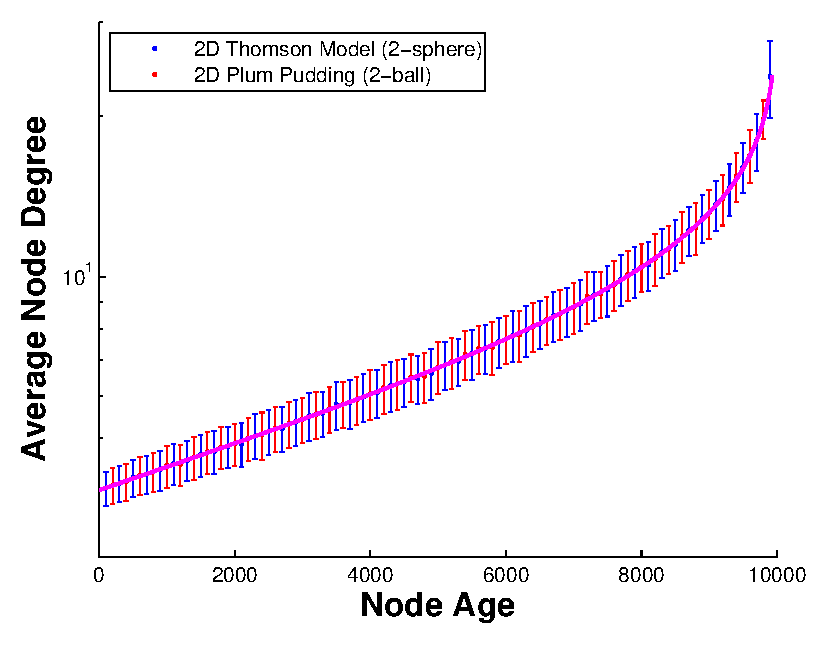
\includegraphics[width=\linewidth]{figures/fig12.pdf}
\caption{\label{degage}Semilogarithmic graph of the mean degree vs the node age for two of the explored models. The magenta line is the theory in Eq. \eqref{ageeq} and the error bars are the standard deviation of the average over 10 simulated networks}
\end{figure}

%once again do we include figures to demonstrate the claim? Which figures to show? They're all pretty much the same since it's the same distribution for every model

\subsection{Betweenness-Degree Relationship}	%this section may not even be necessary...
Betweenness centrality is a common measure of the importance of a node to the propagation of information through a network.
Formally it is the fraction of shortest paths between all node pairs which pass through a given node.
In general we would expect that the nodes with the greatest degree have the highest betweenness since they serve as bridges across the network, meaning many shortest paths between low degree nodes must pass through these high degree nodes.
The existence and subsequent high betweenness of high degree nodes (which can be thought of as hubs in the network) is directly related to the small-world property.
High clustering in networks leads to regions where nodes are highly connected separated from one another.
Short path lengths across the network require these regions to be somehow connected to one another, and this necessitates the existence of hubs to connect the clustered regions.
This means that many low degree nodes aren't necessary for shortest paths across the network since the shortest path will make use of the hubs, leading to higher betweenness for high degree nodes and vice versa.
The variety of models presented here all have the small-world property and share the same degree distribution, and thus we expect they share the same betweenness-degree relationship.

%present figure of betweenness-vs-degree for at least a few of the models?

The main discrepancy between the simulation results and the predictions discussed above appear in the 1 dimensional case.
The high degree nodes in the 1D plum pudding model have much higher betweenness than the high degree nodes in the 1D Thomson model (which is just the OHO model).
The 1D plum pudding model has firm boundary conditions at either edge of the line, and so any shortest path from one side of the line to the other must use ahigh degree node to cross the network.
The OHO model on the other hand has no edge effects and thus the shortest path through the network will go either clockwise or counter-clockwise around the circle, meaning that the shortest paths across the network don't necessarily pass through a select few high degree nodes in the middle (like in the line model).
As we increase the dimension this effect disappears in part because the nodes in higher dimensional spaces are free to move around each other, producing a wider variety of shortest paths than are possible in lower dimensions. 
Thus the discrepancy in betweenness vs. degree in the 1D case can be attributed to the feature that in 1 dimension the nodes behave like a Tonks-Girardeau Gas in that they cannot move past one another.
Although the invariance of the betweenness-degree relationship is not fully established, the higher dimensional models all exhibit the same pattern, indicating that betweenness is not significantly impacted by the space in which the network is embedded as long as the space is sufficiently large to allow nodes to move freely.

\section{Limitations of the Model}
As with any simulation, our models were limited in the degree to which they could accurately represent a "real" scenario while still remaining practically computable.  
In this section, we discuss the necessary shortcomings we have identified in our model, and the effects we believe them to have had on our results.  
However, we first note that the results we have obtained, while certainly biased in one way or another, still appear to accurately represent a genuine trend in the phenomena we investigated, and that the various biases come together to produce what is best characterized as noise, rather than a fundamental flaw.

\subsection{Tolerance of Disequilibrium}
As noted above, we used a gradient-descent method to enforce the even spacing of nodes.  
In order to ensure that the computation halted, we introduced a ceiling on the number of iterations of gradient-descent steps, so that a persistent disequilibrium could not delay the model indefinitely.  
We also introduced a tolerance parameter related to the average inter-node spacing (a function of $N$) such that if all nodes were displaced by less than a certain distance in a single timestep, the gradient-descent algorithm could exit early.  
Both of these steps were necessary to ensure that the use of the model was practically feasible given finite computing resources.

Varying the tolerance, we found that a higher tolerance (resulting in fewer steps before exiting the algorithm) corresponded to decreased displacement of nodes, as was expected.  
Similarly, in cases in which the ceiling on the number of steps was too low (that is, low enough to be encountered frequently), there was less movement than in cases in which the ceiling was high.  
Both of these effects were trades between accuracy and speed; a faster computation meant less displacement, corresponding to a higher clustering coefficient, among other measures.

\subsection{Timestep Size}
For the gradient-descent algorithm, as it was not possible to simulate a truly continuous system, the gradients of each node were calculated and applied in discrete timesteps.  
The size of this timestep tended to be inversely proportional to the time to run a model, so larger timesteps were preferable to smaller ones.  
However, larger timesteps increased the probability of overshooting the equilibrium (an error which would then be remedied in subsequent iterations of or calls to the algorithm), where smaller timesteps would have prevented such movements by recalculating forces more frequently.

Large timesteps, therefore, were also a trade between accuracy and speed, though here, a faster computation meant more displacement.  
This was reflected in a lower clustering coefficient for rather large timesteps, an effect which persisted even for large networks.

\subsection{Force Laws}
Finally, in calculating the gradients for the gradient-descent algorithm, we used a scaling taken from the Coulomb force in an arbitrary number of dimensions: $F \propto \frac{1}{r^{d-1}}$ in a $d$-dimensional space.  
For the $d$-dimensional ball, the ball and the space in which it was embedded were of the same dimension, which as the dimension used there.  
In the case of the $d$-dimensional sphere, however, the dimension of the sphere itself, which was one less than that of the embedding space, was used, which produced results approximately similar to those produced from the $d$-dimensional ball.

However, we found that different force laws produced substantially different arrangements.  %More to follow once we have conclusive data on force/dimension.

\subsection{Error Summary}
Based on informal comparisons to networks using small $N$, we have come to the conclusion that while the error introduced by these factors does affect the properties of the networks, the effects do, to some extent, act against each other.  Increased tolerance results in insufficient movement, while increased timestep size results in extra movement.  With that in mind, and in light of the "growing" nature of our models, it may be appropriate to slightly change our concept of the model.  Rather than converging to a static state, our models instead experience a substantial excitation upon the addition of a new node, but then return to what is akin to a dynamic equilibrium, the activity of its members no longer organized or large.  We believe this is a better analogy for real growing networks, which are rarely truly static.

\section{CONCLUSION}
%Write the conclusion at the end when we have all of the results and figures and even after we've written the introduction, make sure to keep the conclusion short

\bibliography{grownet}

\end{document}

